
\documentclass{article}

% Set this =0 to hide, =1 to show
\def\showanswers{0}

\newcommand{\hide}[1]{
\ifnum\showanswers=1

#1 \vspace{\baselineskip}
\fi

\ifnum\showanswers=0

\vspace{2\baselineskip} \hspace{2cm}
\fi
}
\usepackage{amsmath,amssymb}
\usepackage{lmodern}
\usepackage{iftex}
\ifPDFTeX
\usepackage{graphicx}
  \usepackage[T1]{fontenc}
  \usepackage[utf8]{inputenc}
  \usepackage{textcomp} % provide euro and other symbols
\else % if luatex or xetex
  \usepackage{unicode-math}
  \defaultfontfeatures{Scale=MatchLowercase}
  \defaultfontfeatures[\rmfamily]{Ligatures=TeX,Scale=1}
\fi
% Use upquote if available, for straight quotes in verbatim environments
\IfFileExists{upquote.sty}{\usepackage{upquote}}{}
\IfFileExists{microtype.sty}{% use microtype if available
  \usepackage[]{microtype}
  \UseMicrotypeSet[protrusion]{basicmath} % disable protrusion for tt fonts
}{}
\makeatletter
\@ifundefined{KOMAClassName}{% if non-KOMA class
  \IfFileExists{parskip.sty}{%
    \usepackage{parskip}
  }{% else
    \setlength{\parindent}{0pt}
    \setlength{\parskip}{6pt plus 2pt minus 1pt}}
}{% if KOMA class
  \KOMAoptions{parskip=half}}
\makeatother
\usepackage{xcolor}
\IfFileExists{xurl.sty}{\usepackage{xurl}}{} % add URL line breaks if available
\IfFileExists{bookmark.sty}{\usepackage{bookmark}}{\usepackage{hyperref}}
\hypersetup{
  hidelinks,
  pdfcreator={LaTeX via pandoc}}
\urlstyle{same} % disable monospaced font for URLs
\usepackage{graphicx}
\makeatletter
\def\maxwidth{\ifdim\Gin@nat@width>\linewidth\linewidth\else\Gin@nat@width\fi}
\def\maxheight{\ifdim\Gin@nat@height>\textheight\textheight\else\Gin@nat@height\fi}
\makeatother
% Scale images if necessary, so that they will not overflow the page
% margins by default, and it is still possible to overwrite the defaults
% using explicit options in \includegraphics[width, height, ...]{}
\setkeys{Gin}{width=\maxwidth,height=\maxheight,keepaspectratio}
% Set default figure placement to htbp
\makeatletter
\def\fps@figure{htbp}
\makeatother
\setlength{\emergencystretch}{3em} % prevent overfull lines
\providecommand{\tightlist}{%
  \setlength{\itemsep}{0pt}\setlength{\parskip}{0pt}}
\setcounter{secnumdepth}{-\maxdimen} % remove section numbering
\ifLuaTeX
  \usepackage{selnolig}  % disable illegal ligatures
\fi

\author{}
\date{}

\begin{document}

\begin{center}
    \textbf{ECO432 - mercredi 28 février 2024 de 9h à 11h.}


\end{center}

\begin{center}

\textit{Documents autorisés: dictionnaire papier et feuille A4 annotée}

\end{center}
\bigskip
\bigskip


\hypertarget{exercice-1}{\subsection{Exercice 1}\label{exercice-1}}


Le temps est continu, $t \in [0, +\infty[$. Soit une économie fermée (i.e. qui n’importe ni n’exporte aucun bien), produisant un bien de consommation suivant la fonction de production:

\begin{equation}\label{eq0} Y_t = K_t^{\alpha} L_t^{1-\alpha} \end{equation}

où \( K_t \) est le stock de capital à la date \( t \) et \( L_t \) est la quantité de travail à la date \( t \), supposée croissant au taux exogène \( n > 0 \): \( \forall t \geq 0, \frac{\dot{L}_t}{L_t} = n \). \( \alpha \) est un paramètre compris strictement entre 0 et 1.  Remarquez que le progrès technologique n'apparaît pas dans la fonction de production ci-dessus -- il apparaîtra dans l'équation (\ref{eq1}) ci-dessous.

L'output $Y_t$ peut être soit consommé, soit investi:
\begin{equation}Y_t=C_t+I_t \end{equation} où $I_t$ est l'investissement physique mesuré en unités de consommation. 

% Chaque unité de bien de consommation peut être soit consommée, soit transformée en \( q_t > 0 \) unités de bien capital. Ainsi, l’équation d’accumulation du capital est :
% Contrairement au modèle de Solow ordinaire, nous supposons ici l’existence de deux biens distincts : le bien de consommation, et le bien capital. Le bien capital est produit à partir du bien de consommation, par une technologie linéaire et en situation de concurrence pure et parfaite.

% Chaque unité de bien de consommation peut être soit consommée, soit transformée en \( q_t > 0 \) unités de bien capital.


Les agents de l’économie ont un taux d’épargne constant \( s \in]0,1] \) et $I_t = s Y_t $.  Ainsi, l’équation d’accumulation du capital est :

\begin{equation}\label{eq1}
    \dot{K}_t = -\delta K_t + q_t I_t 
\end{equation}
où \( \delta > 0 \) est le taux instantané de dépréciation du capital, et où $q_t I_t$ représente l'investissement mesuré en unités efficaces. Remarquez que l'investissement, mesuré en unités de consommation, $I_t$, est multiplié par un terme qui représente la qualité des biens d'investissement nouvellement produits, $q_t$. Ce terme $q_t$ est appelé « productivité spécifique à l’investissement » et il augmente de manière exponentielle : $q_t = q_0 \exp(g_q t)$ avec $q_0 > 0$ et $g_q > 0$ exogènes. L'augmentation de $q_t$ au fil du temps reflète les changements technologiques dans la production de nouveaux biens d'équipement.


% The improvement in the quality of capital goods
% reflected in increasing values of qt is the driving force
% behind investment-specific technological change.
% \begin{equation}\label{eq2}
%    I_t = s Y_t 
% \end{equation}
% où \( \delta > 0 \) est le taux instantané de dépréciation du capital, et où \( q_t \) est le terme dit de « productivité spécifique à l’investissement » et qui augmente exponentiellement : \( q_t = q_0 \exp(g_q t) \) avec \( q_0 > 0 \) et \( g_q > 0 \) exogènes.   When q(t) is high, the same investment expenditure translates into a greater increase in the capital stock. Il existe à la date 0 \( K_0 > 0 \) unités de capital et la population est à \( L_0 > 0 \).
% Notice that in (\ref{eq0}) there is no term technological progress that 

% Final output, less adjustment costs, $a$ (to be discussed below), can be used for three purposes: consumption, $c$, investment in structures, $i_s$, and investment in equipment, $i_e$.
% \begin{equation}y=c+I \end{equation}

\begin{enumerate}
\item Par définition, sur un chemin de croissance équilibrée, le capital par travailleur doit croître à un taux constant.  Démontrer qu'il n'y a qu'un seul taux de croissance possible du ratio capital-travail qui est cohérent avec une croissance équilibrée. (Aide: pour répondre à cette question, commencez par exprimer l'équation (\ref{eq1}) en termes de capital par travailleur)

\item Soit \( \gamma \in \mathbb{R} \). On note  \( \hat{k}_t = \frac{K_t}{(q_t)^{\gamma} L_t} \) où $\hat{k}_t$ est le ratio capital-travail “normalisé." En utilisant (\ref{eq1}), calculer \( \frac{\dot{\hat{k}}_t}{\hat{k}_t} \) en fonction de \( K_t \), \( L_t \), \( q_t \) et des paramètres.

 \item Trouvez la valeur de \( \gamma \) pour laquelle \( \hat{k}_t \) obéit à une équation différentielle autonome (dans cette équation, 
$q_t$ n'apparaît pas).   \item Trouvez l'état stationnaire $\hat{k}^{\ast}$ pour \( \hat{k}_t \).  \item Avec un graphique, démontrer que, en commençant avec n'importe quel \( \hat{k}_0 \), le ratio capital-travail normalisé dans cette économie converge vers \( \hat{k}^{\ast}>0 \). Montrer que à long terme le ratio capital-travail \( \frac{K}{L} \) croît à un taux constant (à préciser). Montrer également que le taux de croissance du PIB par tête tend vers une certaine limite \( g_y \) (à préciser).


 \item Dans le modèle de base de Solow, le bien capital et le bien de consommation ont le même prix car pour produire une nouvelle machine, une unité de consommation est nécessaire. Dans ce modèle, ce n'est plus le cas. Quel est le prix du bien capital en termes du bien de consommation ? 
\item Ce modèle de croissance est-il compatible avec le quatrième fait stylisé de Kaldor, selon lequel le ratio capital/PIB n’a pas de tendance de long terme ? Si ce n'est pas le cas, expliquez l'intuition. Et si vous preniez plutôt le ratio entre la valeur du capital ($K_t$ fois le prix du bien capital) et le PIB, serait-il stable à long terme ?
\item Le modèle présenté est-il cohérent avec la figure ci-dessous ?
\bigskip 

\begin{figure}
  \centering
  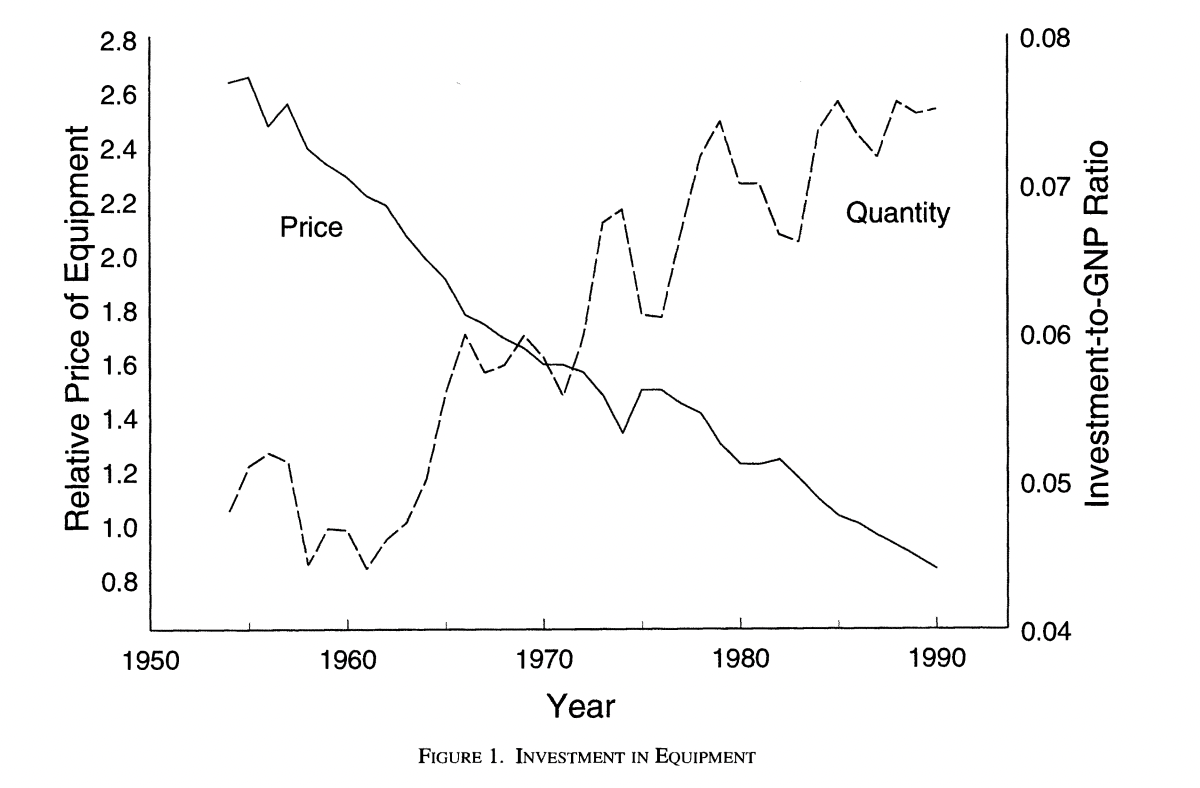
\includegraphics[width=0.6\textwidth]{pi.png}
  \caption{ prix des équipements et ratio investissement-en-équipement/produit national brut : Greenwood, et al, 1997}
  \label{fig:example}
\end{figure}
\newpage 


\hypertarget{mcq}{\subsection{Exercice 2: questions de cours}\label{mcq}}


\begin{enumerate}
    \tightlist

\item Laquelles des assertions suivantes est fausse ?

\begin{enumerate}
\tightlist
\item
  la propension marginale à consommer des consommateurs est comprise
  entre 0 et 1
\item
  la consommation des consommateurs ricardiens réagit au taux d'intérêt
  réel
\item
  si tous les consommateurs sont keynésiens, une baisse du taux
  d'intérêt réel ne stimule pas la demande agrégée
\item
  la banque centrale stabilise la demande en influant sur le taux
  d'intérêt réel
\end{enumerate}

\item A la suite d'un choc inconnu, on a observé une baisse de la
production accompagnée d'une augmentation de l'inflation. Après
plusieurs périodes, la production est revenue à son niveau d'origine
mais l'inflation est restée à un niveau plus haut. Quel type d'événement
est compatible avec cette observation ?

\begin{enumerate}
\tightlist
\item
  Un choc négatif persistent de la production et un choc négatif
  temporaire de la demande
\item
  Un choc négatif temporaire de la production et un choc postif
  persistent de la demande
\item
  Un choc positif temporaire de la production et un choc négatif
  persistent de la demande
\item
  Un choc positif persistent de la production et un choc négatif
  temporaire de la demande
\end{enumerate}

\end{enumerate}


\hypertarget{mcq}{\subsection{Exercice 3: marché du travail}\label{exo3}}


On suppose que les firmes produisent avec une technologie linéaire
\(Y_t = L_t Z_t\) où \(L_t\) est le nombre d'heures travaillées, et
\(Z_t\) un choc de productivité. Le salaire horaire est \(W_t\).

\begin{enumerate}
    
\item Quel est le coût marginal de la production?

\end{enumerate}

Les travailleurs maximisent chaque période une fonction d'utilité \(V(C_t,L_t) = \frac{{C_t}^{1-\sigma}}{1-\sigma} - \frac{1}{\xi}{L_t}^{\xi}\)
    où \(C_t\) est la consommation et \(L_t\) le nombre d'heures travaillées  et \(\xi\) un paramètre positif. On note \(P_t\) le niveau des prix.

\begin{enumerate}

\setcounter{enumi}{1}

\item Écrire la contrainte de budget intratemporelle des travailleurs et déterminer leur offre de travail à l'équilibre.
    
\item Quel est l'équilibre sur le marché du travail? Représentation
    graphique.
    
\item On suppose maintenant que les firmes fixent leur prix optimal \(P^{\star}_t\) en intégrant une marge \(\mu\) sur le coût marginal. En supposant les prix parfaitement flexibles calculer l'équilibre de
long terme pour les différentes variables macroéconomiques. Commenter l'effet de la productivité \(Z\) et du taux de marge \(\mu\) sur \(Y\) et \(L\).
    
\end{enumerate}

\hypertarget{exo4}{\subsection{Exercice 4: principe de Taylor}\label{exo4}}


On considère ici une économie loglinéarisée caractérisée par les courbes
IS et PC suivantes:

\begin{equation}\phantomsection\label{eq-is}{y_t = y_{t+1} - \sigma \left( i_t - \pi_{t+1} \right) + e^{\pi}_t}\end{equation}
\begin{equation}\phantomsection\label{eq-pc}{\pi_t = \kappa (y_t - e^y_t)  + \beta \pi_{t+1}}\end{equation}

où \(\pi_t\) dénote l'inflation, \(y_t\) la production, \(i_t\) le taux
d'intérêt et où \(\sigma\) et \(\kappa\) sont des paramètres réels
positifs et où \(\beta \in ]0,1[\) est le facteur d'escompte.

Les variables \(e^{\pi}_t\) et \(e^{y}_t\) sont respectivement des chocs
de demande et d'offre.\footnote{Ici, la courbe de Philips provient de la
  fixation des prix par des entreprises en compétitions monopolistique,
  qui optimisent leur profits futurs plutôt qu'instantané. On parle de
  courbe de Philips augmentée par les anticipations.}. Ils sont pris
comme exogènes et on les suppose bornés. On suppose qu'il n'y a pas
d'incertitude sur la valeur des chocs futurs, de sorte qu'on peut
omettre les symboles d'espérance et considérer toutes leurs valeurs
comme connues.

La banque centrale suit une règle pour fixer son taux d'intérêt:
\begin{equation}\phantomsection\label{eq-taylor}{i_t = i^{\star} + \varphi_y (y_t - e^{\pi}_t) + \varphi_\pi (\pi_t - \pi^{\star})}\end{equation}

avec la cible d'inflation égale au taux d'intérêt cible:
\(i^{\star}=\pi^{\star}\).

On dit qu'une règle de Taylor satisfait le principe de Taylor, si en
réponse à un choc de demande permanent ayant pour effet d'augmenter
l'inflation d'1\%, la banque centrale augmente le taux d'intérêt de plus
d'1\%.

\begin{enumerate}

\item  Définir deux matrices A, B telles que: \[z_{t+1} = A z_t + B e_t\] où \(z_t=(\pi_t, y_t)\) et \(e_t = (e^{\pi}_t, e^{y}_t)\)
\item   Montrer que les niveaux d'inflation et de production sont uniquement déterminés à toutes les dates \(t\geq 0\) si \[\varphi_{\pi} + \frac{1-\beta}{\kappa} \varphi_{y}> 1\] Cela   correspond-il a une banque centrale plus active ou plus passive   vis-à-vis de l'inflation ? Comparer avec le principe de Taylor.
\end{enumerate}


\end{document}

